\documentclass[12pt,a4paper]{article}

\usepackage[brazil]{babel}
\usepackage[T1]{fontenc}
\usepackage[utf8]{inputenc}
\usepackage{geometry}
\geometry{margin=2.5cm}
\usepackage{graphicx}
\usepackage{booktabs}
\usepackage{siunitx}
\usepackage{hyperref}
\usepackage{caption}
\usepackage{amsmath}

\sisetup{output-decimal-marker={,}, group-separator={.}}

\title{Previsão de tráfego de rede com LSTM\\
\large MC833A -- Programação em Redes de Computadores}
\author{Lucas félix\\RA: 247064}

\begin{document}
\maketitle

\begin{abstract}
Este relatório apresenta a análise exploratória e o modelamento preditivo do throughput
em dois traces do projeto MAWI (WIDE, Japão), medidos no mesmo dia da semana e horário
(sábado, 10 de fevereiro, 14:00 JST) com 17 anos de diferença: 2007 e 2024.
Utilizamos redes neurais recorrentes do tipo LSTM para prever o throughput do segundo
seguinte a partir de janelas deslizantes de histórico, comparando desempenho no mesmo
ano e em generalização cruzada entre eras.
\end{abstract}

\section{Introdução}

A previsão do volume de tráfego em links de backbone é relevante para planejamento de
capacidade, detecção de anomalias e balanceamento de carga. Neste projeto, analisamos
e prevemos o tráfego observado em um ponto de medição real do MAWI, comparando a
Internet medida em 2007 e em 2024 sob condições de calendário semelhantes (mesmo dia da
semana e horário), de modo a destacar mudanças de escala e de comportamento ao longo do
tempo, e não apenas variações intradiárias.

O trabalho divide-se em análise exploratória de dados (EDA) e modelamento com LSTM.
Os resultados numéricos e gráficos foram obtidos nos notebooks
\texttt{01\_EDA.ipynb} e \texttt{02\_LSTM.ipynb}, executados no Google Colab com
TensorFlow/Keras. Ressaltamos que os dados correspondem a \emph{um} link, em \emph{um}
intervalo de 15 minutos em um sábado à tarde; conclusões amplas sobre ``a Internet''
devem ser evitadas.

\section{Descrição geral e metodologia}

O fluxo de trabalho seguiu o roteiro fornecido na disciplina:
\begin{enumerate}
  \item Carregar séries pré-processadas em Parquet (agregação a partir dos PCAP originais
        do MAWI, sem necessidade de reprocessar os traces brutos).
  \item Explorar throughput total, TCP e UDP, e a distribuição de tamanhos de pacotes.
  \item Construir séries de throughput a 1\,s, dividir temporalmente em treino (80\%)
        e teste (20\%), normalizar com \texttt{MinMaxScaler} ajustado apenas no treino,
        e gerar janelas deslizantes de 10, 20 e 30 segundos.
  \item Treinar, para cada ano, uma LSTM enxuta (32 unidades) com saída densa escalar,
        avaliar pelo erro quadrático médio (MSE) no teste e salvar o melhor modelo por
        ano conforme a menor perda de validação.
  \item Avaliar generalização cruzada: modelos treinados em 2007 e 2024 testados em ambos
        os anos.
\end{enumerate}

Para reprodutibilidade, fixamos a semente aleatória em 42 (\texttt{fixar\_sementes}).

\section{Dados}

Utilizamos os traces MAWI \texttt{200702101400} (2007) e \texttt{202402101400} (2024),
cada um com cerca de 900\,s de duração. Os arquivos Parquet incluem série temporal em
bins de 10\,ms (bytes e pacotes por protocolo), histogramas de tamanho de pacote e
resumos em JSON.

A Tabela~\ref{tab:resumo} resume grandezas agregadas dos dois traces. O crescimento de
volume entre 2007 e 2024 é marcante: quase dez vezes mais pacotes e throughput médio
cerca de 13 vezes maior. O tráfego permanece majoritariamente TCP em bytes, mas a
participação de UDP e IPv6 aumenta em 2024; o tamanho médio de pacote também cresce.

\begin{table}[htbp]
  \centering
  \caption{Resumo comparativo dos traces MAWI (sábado 10/02, 14:00 JST).}
  \label{tab:resumo}
  \begin{tabular}{lrr}
    \toprule
    Grandeza & 2007 & 2024 \\
    \midrule
    Duração (s) & 900,3 & 899,8 \\
    Pacotes (milhões) & 14,49 & 138,79 \\
    Volume (GB) & 10,61 & 138,22 \\
    Throughput médio (Mbps) & 94,3 & 1228,9 \\
    Tamanho médio do pacote (B) & 732,5 & 995,9 \\
    \% bytes TCP / UDP & 97,2 / 2,1 & 88,1 / 7,9 \\
    \% pacotes IPv6 & 0,7 & 9,0 \\
    \bottomrule
  \end{tabular}
\end{table}

\section{Análise exploratória de dados}

\subsection{Estatísticas descritivas do throughput}

A Tabela~\ref{tab:estatisticas} apresenta média, desvio-padrão, mínimo, quartis e máximo
do throughput por segundo (Mbps), separando tráfego total, TCP e UDP. Em 2007, a série
total é relativamente estável (desvio-padrão de \SI{8,58}{Mbps} frente a média de
\SI{94,29}{Mbps}); TCP concentra quase todo o volume e UDP permanece em torno de
\SI{2}{Mbps}. Em 2024, a média total salta para \SI{1229,11}{Mbps}, mas o
desvio-padrão (\SI{626,23}{Mbps}) e o máximo (\SI{5591,12}{Mbps}) indicam forte
variabilidade e picos abruptos. O UDP passa a ter média de \SI{96,74}{Mbps} e picos
acima de \SI{343}{Mbps}, refletindo aplicações mais dependentes de datagramas (vídeo,
DNS, QUIC e serviços similares).

\begin{table}[htbp]
  \centering
  \caption{Estatísticas descritivas do throughput por segundo (Mbps).}
  \label{tab:estatisticas}
  \small
  \begin{tabular}{llrrrrrrr}
    \toprule
    Ano & Série & Média & Desv. & Mín. & Q1 & Med. & Q3 & Máx. \\
    \midrule
    2007 & Total & 94,29 & 8,58 & 66,64 & 88,41 & 94,37 & 99,86 & 123,73 \\
    2007 & TCP   & 91,63 & 8,54 & 64,09 & 85,88 & 91,66 & 97,14 & 121,41 \\
    2007 & UDP   &  2,01 & 0,33 &  1,40 &  1,81 &  1,92 &  2,10 &   5,15 \\
    2024 & Total & 1229,11 & 626,23 & 483,00 & 818,46 & 1091,54 & 1454,95 & 5591,12 \\
    2024 & TCP   & 1082,42 & 627,09 & 358,21 & 677,27 & 937,85 & 1313,89 & 5442,49 \\
    2024 & UDP   &   96,74 &  33,26 &  46,88 &  73,77 &  91,34 &  110,94 &  343,38 \\
    \bottomrule
  \end{tabular}
\end{table}

\subsection{Gráficos}

A Figura~\ref{fig:throughput} mostra o throughput total por segundo ao longo dos
15 minutos. Em 2007 a série oscila em faixa estreita; em 2024 há patamares mais altos
intercalados com quedas e picos isolados, típicos de rajadas e de mix de aplicações
mais agressivo em largura de banda.

\begin{figure}[htbp]
  \centering
  \includegraphics[width=\linewidth]{throughput_temporal.png}
  \caption{Throughput total por segundo (Mbps) em 2007 (esquerda) e 2024 (direita).}
  \label{fig:throughput}
\end{figure}

A Figura~\ref{fig:hist-vazao} compara as distribuições de throughput de TCP e UDP. Em
2007, TCP e UDP ocupam escalas muito diferentes (UDP concentrado em valores baixos). Em
2024, ambos os protocolos apresentam distribuições mais espalhadas, com UDP ganhando
massa em faixas intermediárias e altas.

\begin{figure}[htbp]
  \centering
  \includegraphics[width=\linewidth]{histograma_throughput_tcp_udp.png}
  \caption{Histogramas do throughput (Mbps) de TCP e UDP por segundo.}
  \label{fig:hist-vazao}
\end{figure}

A Figura~\ref{fig:hist-tam} exibe a distribuição do tamanho dos pacotes. Em 2024 há
maior presença de pacotes grandes (coerente com o aumento do tamanho médio) e mudança
no perfil UDP/TCP, compatível com evolução de pilhas de protocolo e padrões de
fragmentação/MTU na Internet medida.

\begin{figure}[htbp]
  \centering
  \includegraphics[width=\linewidth]{histograma_tamanho_pacotes.png}
  \caption{Distribuição do tamanho de pacotes (TCP e UDP).}
  \label{fig:hist-tam}
\end{figure}

\subsection{Comentários}

Entre 2007 e 2024 observamos crescimento de escala, maior heterogeneidade de tráfego
(UDP e IPv6) e dinâmica temporal mais ``espiky'' em 2024. Esses fatores antecipam que
modelos preditivos calibrados em um ano podem falhar ao extrapolar para o outro, pois
mudam não só a média, mas a variância e a presença de eventos extremos.

\section{Modelamento preditivo}

\subsection{Abordagem LSTM}

A tarefa é prever o throughput do \emph{próximo} segundo a partir dos
\texttt{look\_back} valores anteriores. Cada amostra de entrada tem forma
$(\texttt{look\_back}, 1)$; a saída é um valor escalar. A rede é uma camada LSTM com
32 unidades seguida de camada densa linear. Otimizador Adam, função de perda MSE.
Treinamento com até 50 épocas, \texttt{batch\_size} 32, 10\% do treino reservado para
validação temporal e \texttt{EarlyStopping} (\texttt{patience}=5,
\texttt{restore\_best\_weights}=True).

A divisão treino/teste respeita a ordem temporal (80\%/20\%). A normalização
\texttt{MinMaxScaler} é ajustada somente nos pontos de treino e aplicada ao conjunto
inteiro antes da criação das janelas, evitando vazamento de informação do futuro.

Testamos janelas de 10, 20 e 30\,s. A melhor configuração por ano foi escolhida pela
menor \texttt{val\_loss}, não pelo teste. Os modelos finais foram salvos como
\texttt{lstm\_2007.keras} e \texttt{lstm\_2024.keras}.

\subsection{Resultados por tamanho de janela}

A Tabela~\ref{tab:mse-janela} lista MSE e RMSE relativo à média no teste. Em 2007, a
janela de 20\,s obteve menor MSE (\SI{32,29}{Mbps^2}) e RMSE/média de 5,91\%, ligeiramente
melhor que a persistência (último valor observado), com 6,43\%. Em 2024, a janela de
30\,s foi a melhor (MSE \SI{39277,54}{Mbps^2}, RMSE/média 18,09\%), superando a
persistência (18,59\%), porém com erro absoluto muito maior devido à escala da série.

\begin{table}[htbp]
  \centering
  \caption{MSE no conjunto de teste por ano e tamanho de janela (\texttt{look\_back}).}
  \label{tab:mse-janela}
  \begin{tabular}{crrr}
    \toprule
    Ano & Janela (s) & MSE (Mbps$^2$) & RMSE/média LSTM (\%) \\
    \midrule
    2007 & 10 & 40,67 & 6,63 \\
    2007 & 20 & 32,29 & 5,91 \\
    2007 & 30 & 32,72 & 5,95 \\
    2024 & 10 & 66760,66 & 23,58 \\
    2024 & 20 & 42095,48 & 18,72 \\
    2024 & 30 & 39277,54 & 18,09 \\
    \bottomrule
  \end{tabular}
\end{table}

A Figura~\ref{fig:lstm-t1} ilustra o primeiro experimento em 2007 (janela 10\,s): curva
real versus prevista no teste e evolução da perda de treino e validação. O modelo
acompanha bem trechos estáveis e apresenta atraso em variações mais rápidas.

\begin{figure}[htbp]
  \centering
  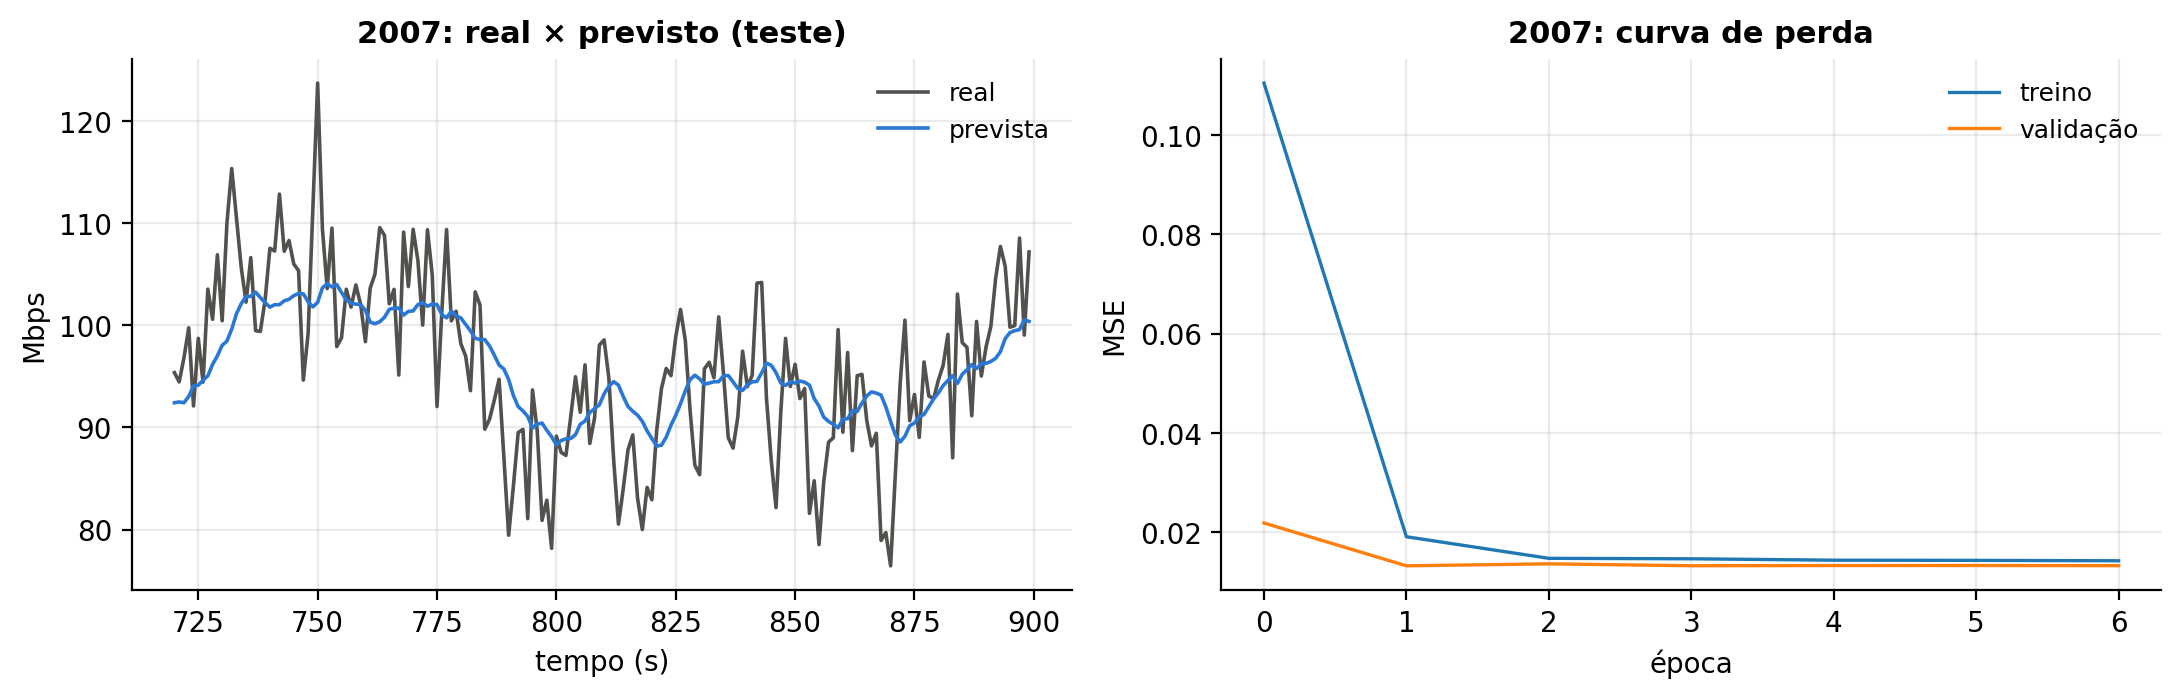
\includegraphics[width=\linewidth]{lstm_2007_t1.png}
  \caption{2007, janela 10\,s: throughput real $\times$ previsto no teste (esquerda) e
    curvas de perda MSE (direita).}
  \label{fig:lstm-t1}
\end{figure}

A Figura~\ref{fig:lstm-melhor} mostra o desempenho dos melhores modelos por ano (20\,s
para 2007, 30\,s para 2024). Em 2007 a previsão segue de perto a série real. Em 2024 o
modelo captura tendências de médio prazo, mas subestima ou atrasa picos acentuados,
onde a dinâmica excede o que uma janela curta e uma única variável explicam.

\begin{figure}[htbp]
  \centering
  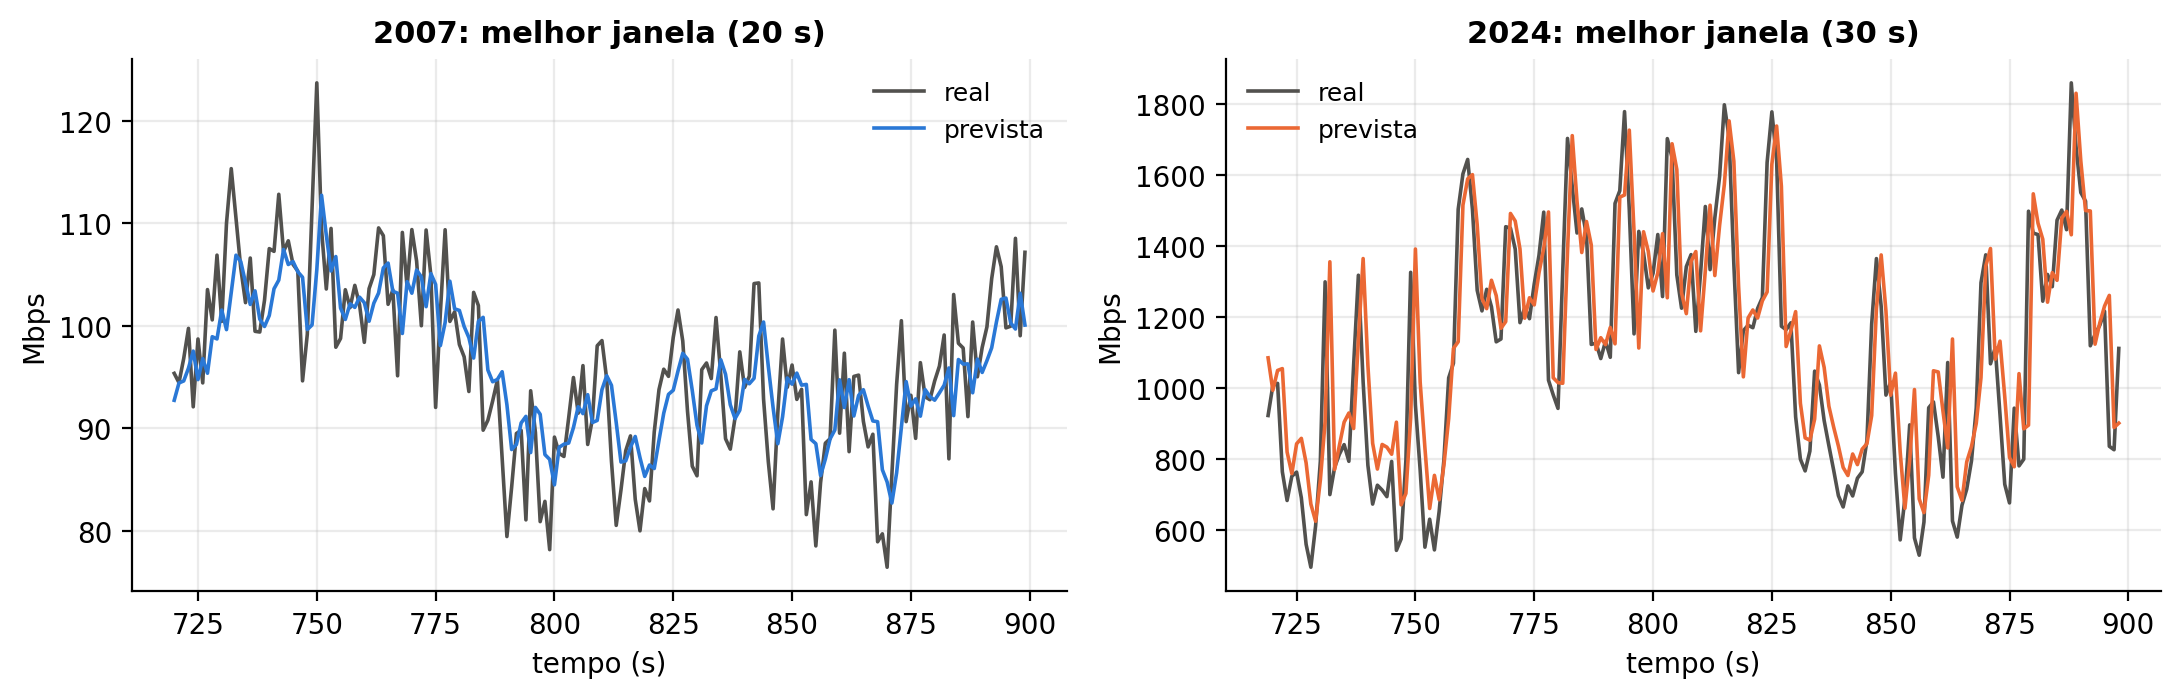
\includegraphics[width=\linewidth]{lstm_melhor_real_previsto.png}
  \caption{Melhor janela por ano: real $\times$ previsto no conjunto de teste.}
  \label{fig:lstm-melhor}
\end{figure}

\section{Comparação 2007 $\times$ 2024 (modelos cruzados)}

A Tabela~\ref{tab:matriz} e a Figura~\ref{fig:matriz} resumem o teste de cada modelo
no trace do ano de treino e no trace do outro ano. Na diagonal, 2007$\rightarrow$2007
mantém RMSE/média de 5,91\%; 2024$\rightarrow$2024 fica em 18,09\%. Fora da diagonal,
o desempenho colapsa: 2007$\rightarrow$2024 atinge 85,53\% e 2024$\rightarrow$2007
315,20\% de RMSE/média, indicando que os modelos aprendem estatísticas locais do ano
de treino (escala, amplitude de rajadas) e não transferem entre domínios.

\begin{table}[htbp]
  \centering
  \caption{Matriz modelo treinado $\times$ ano de teste.}
  \label{tab:matriz}
  \begin{tabular}{ccrrr}
    \toprule
    Modelo & Teste & MSE (Mbps$^2$) & RMSE (Mbps) & RMSE/média (\%) \\
    \midrule
    2007 & 2007 & 32,29 & 5,68 & 5,91 \\
    2007 & 2024 & 878531,74 & 937,30 & 85,53 \\
    2024 & 2007 & 91807,45 & 303,00 & 315,20 \\
    2024 & 2024 & 39277,54 & 198,19 & 18,09 \\
    \bottomrule
  \end{tabular}
\end{table}

\begin{figure}[htbp]
  \centering
  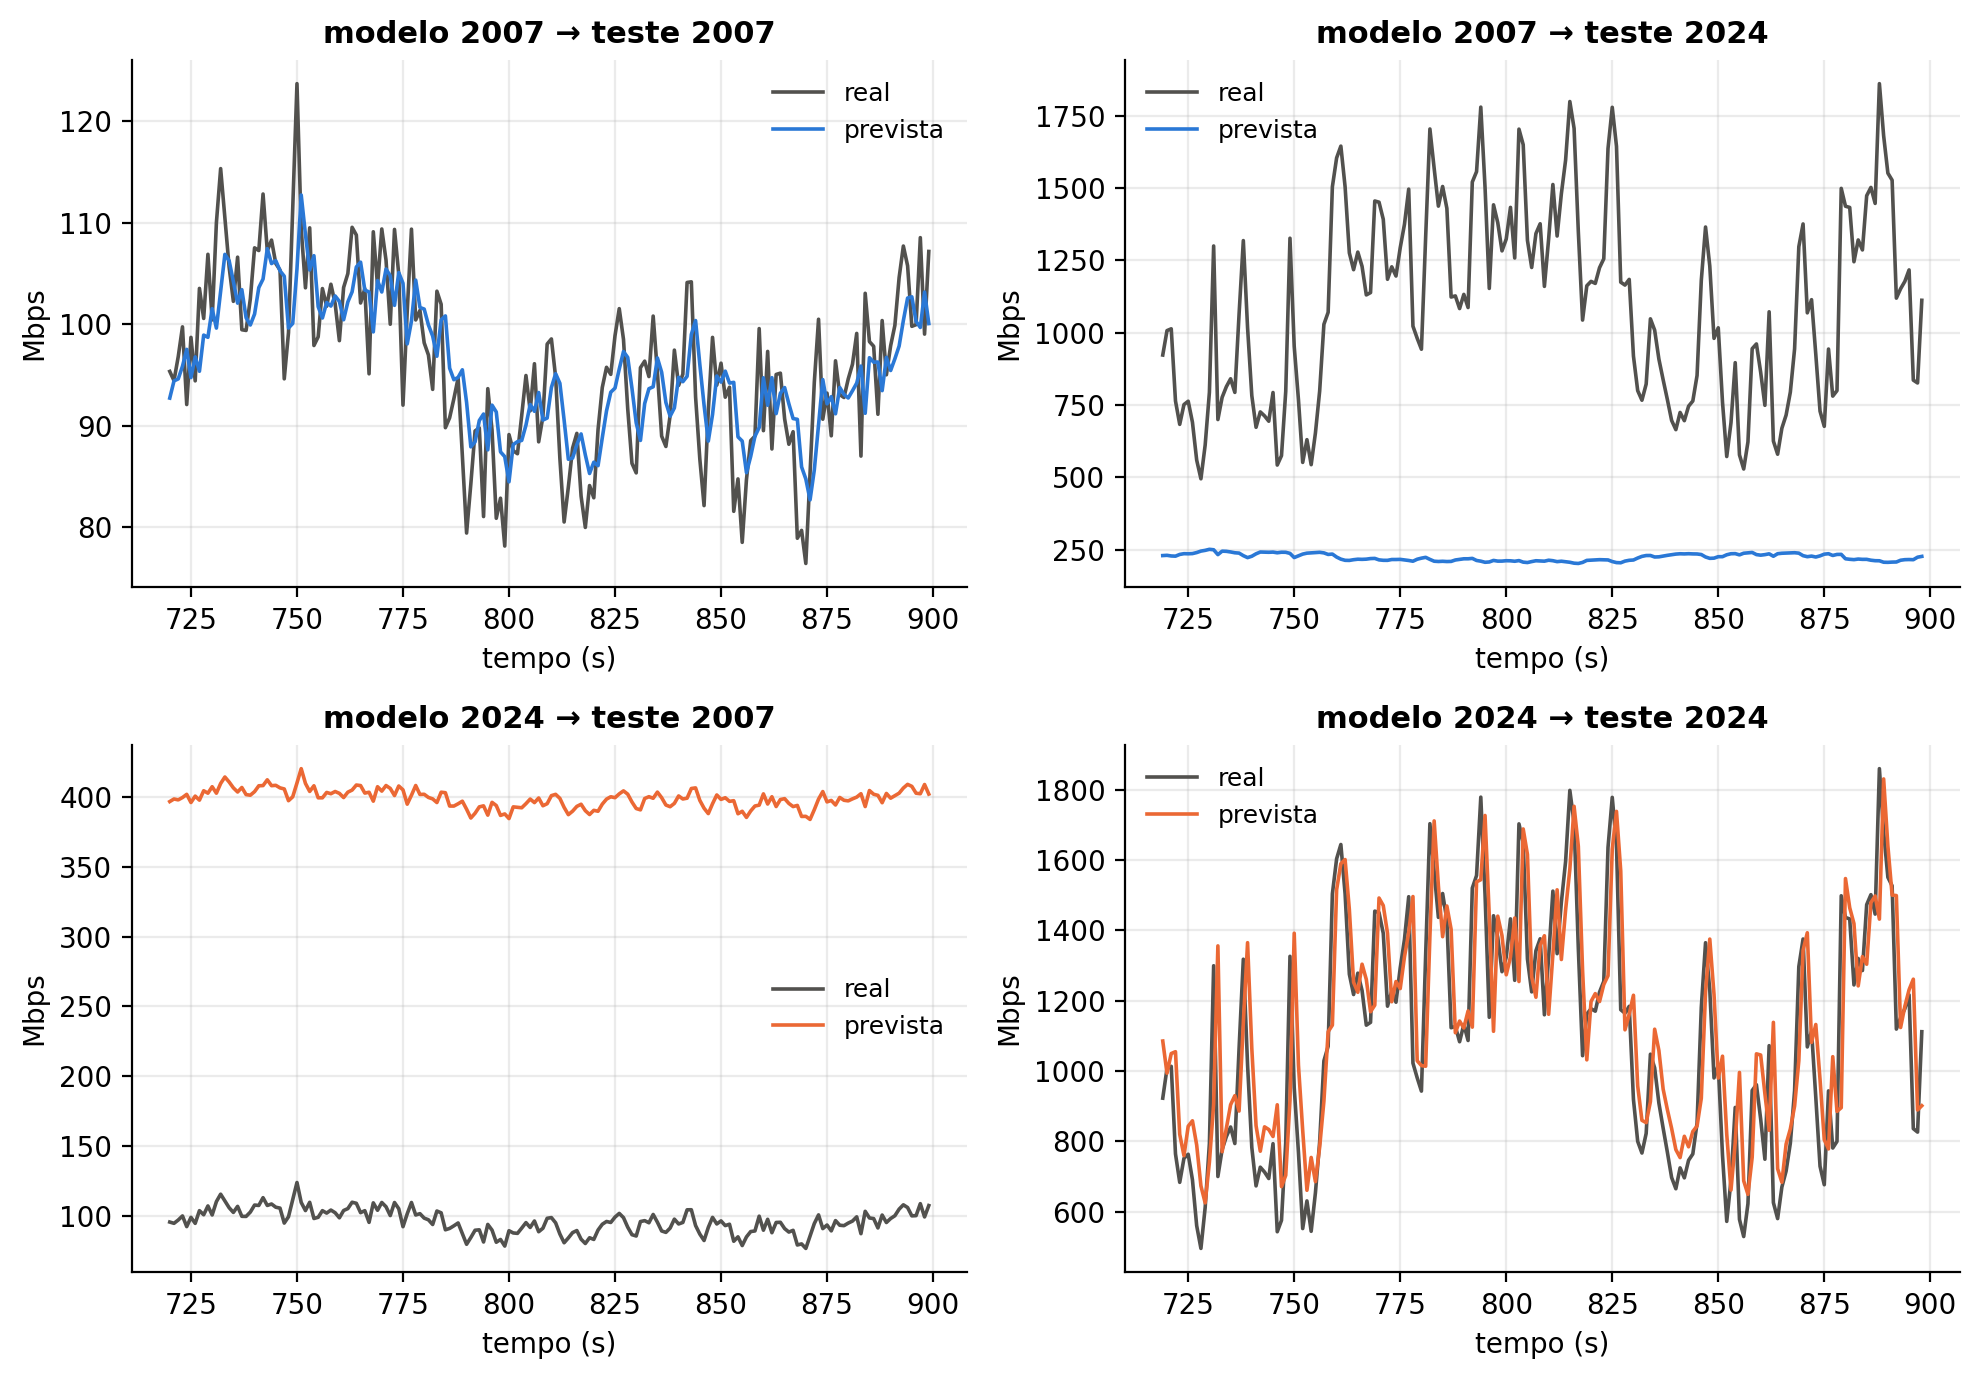
\includegraphics[width=0.85\linewidth]{matriz_modelo_teste.png}
  \caption{Throughput real (cinza) e previsto (cor do modelo) para as quatro combinações
    treino$\times$teste.}
  \label{fig:matriz}
\end{figure}

\section{Discussão crítica}

O bom desempenho em 2007 está alinhado a uma série mais estacionária em escala reduzida:
rajadas existem, mas a LSTM com janela de 20\,s consegue aproximar a continuidade temporal.
Em 2024, picos isolados e maior variância violam a hipótese implícita de suavidade;
o MSE penaliza fortemente subestimação de picos, inflando o erro. A normalização por
MinMax no treino de cada ano não alinha distribuições entre 2007 e 2024, o que explica
a falha cruzada: um modelo treinado em escala normalizada de 2024 projeta valores
incompatíveis quando o scaler de 2007 é reutilizado (e vice-versa).

Do ponto de vista de redes, o aumento de UDP e de pacotes maiores sugere mix de
aplicações distinto (streaming, DNS recursivo, possíveis fluxos bulk TCP paralelos).
Picos podem corresponder a transferências curtas ou eventos de agregação no ponto de
medição, não necessariamente a anomalias maliciosas, mas funcionam como ``teste de
estresse'' para preditores de curto prazo.

\textbf{Limitações:} uma única variável (throughput total), janelas curtas, arquitetura
mínima e um par de traces. \textbf{Vantagens:} pipeline reprodutível, baseline de
persistência, comparação explícita entre eras.

\textbf{Trabalho futuro:} incluir séries multivariadas (TCP/UDP separados), janelas
adaptativas, modelos com atenção (Transformer), ensemble com modelos estatísticos
(ARIMA/Prophet), e validação em múltiplos dias e pontos MAWI.

\section{Conclusão}

A EDA mostrou crescimento massivo de tráfego e maior irregularidade em 2024 em relação
a 2007. As LSTMs treinadas por ano preveem razoavelmente o próximo segundo no mesmo ano,
especialmente em 2007, com melhoria sobre a persistência na configuração escolhida.
A generalização entre anos é inviável com o setup proposto, evidenciando mudança de
regime entre as medições. O estudo reforça que previsão de tráfego deve considerar
estacionariedade local, escala e características de protocolo, além de métricas relativas
quando se comparam períodos com médias muito distintas.

\end{document}
